% Requires: \usepackage{graphicx,booktabs}
% Paths are relative to the repository root.
\begin{figure}[t]
  \centering
  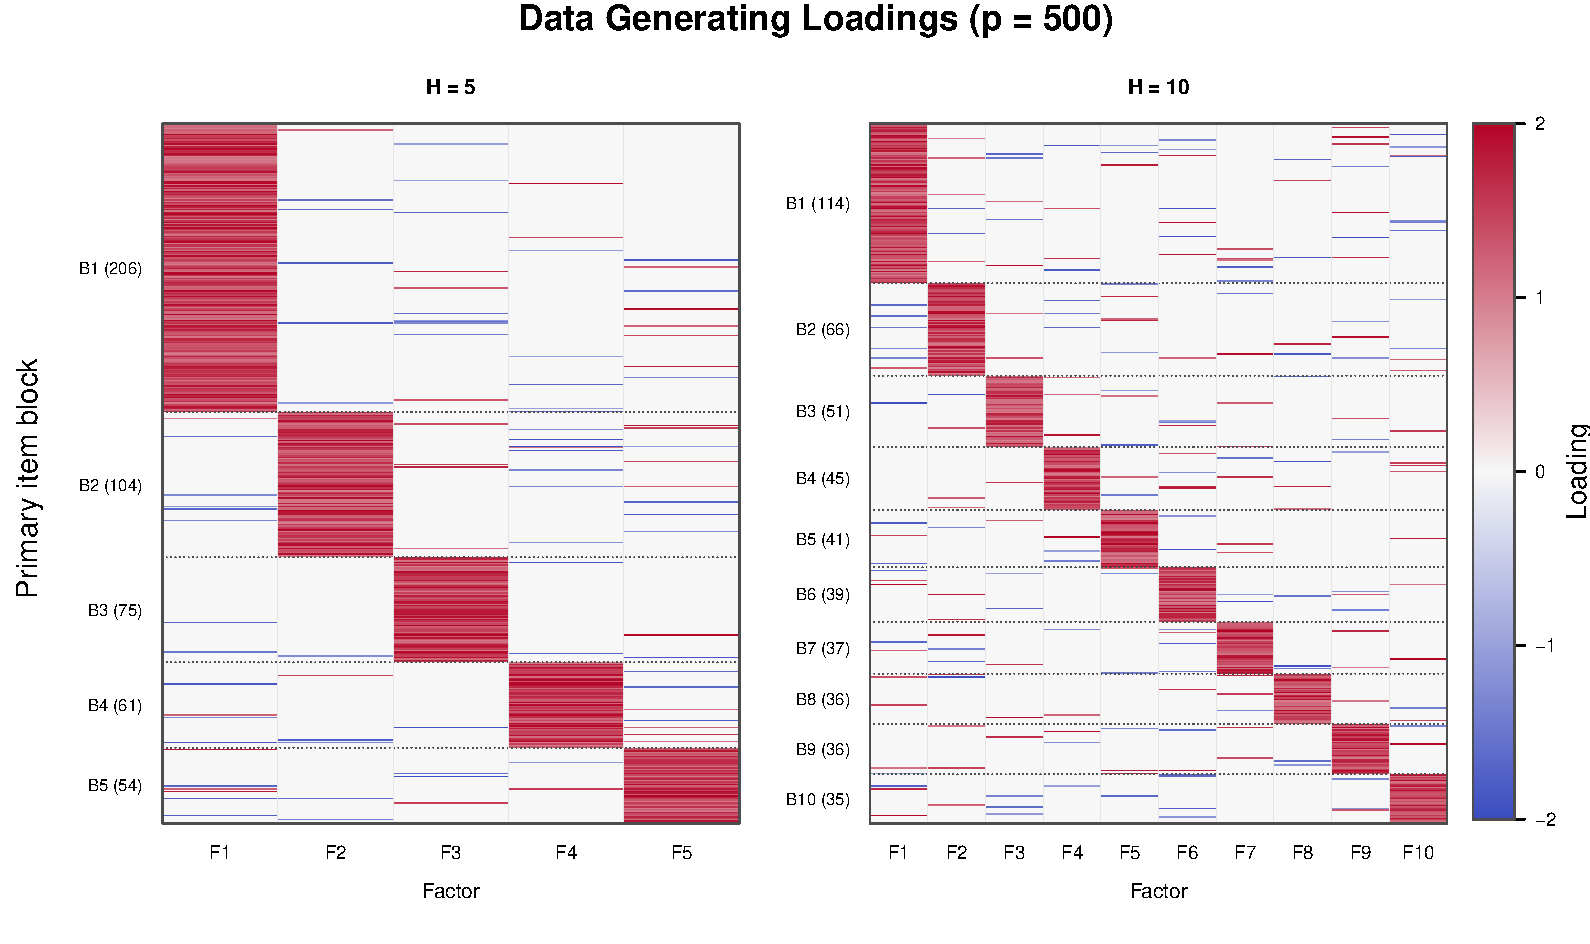
\includegraphics[width=\linewidth]{results/selected_plots/sample_size/paper_simulation_section/fig_data_generating_loadings.pdf}
  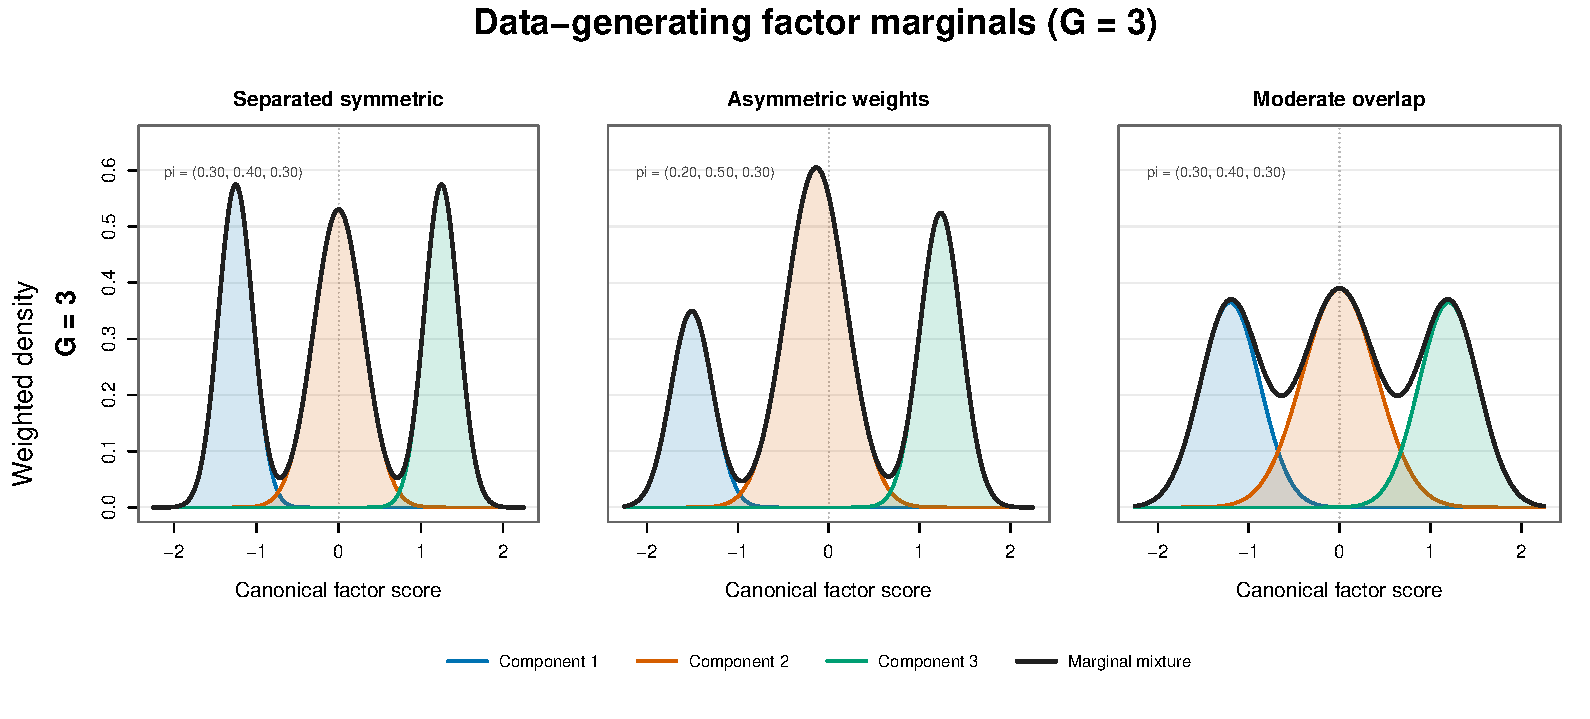
\includegraphics[width=\linewidth]{results/selected_plots/sample_size/paper_simulation_section/fig_data_generating_mixtures.pdf}
  \caption{Data-generating loading structures and latent factor mixture distributions. Top: loading matrices for $p=500$ and $H\in\{5,10\}$. Bottom: representative three-component factor marginals under separated symmetric, asymmetric-weight, and moderate-overlap configurations.}
  \label{fig:loadings_clusters}
\end{figure}

\begin{figure*}[t]
  \centering
  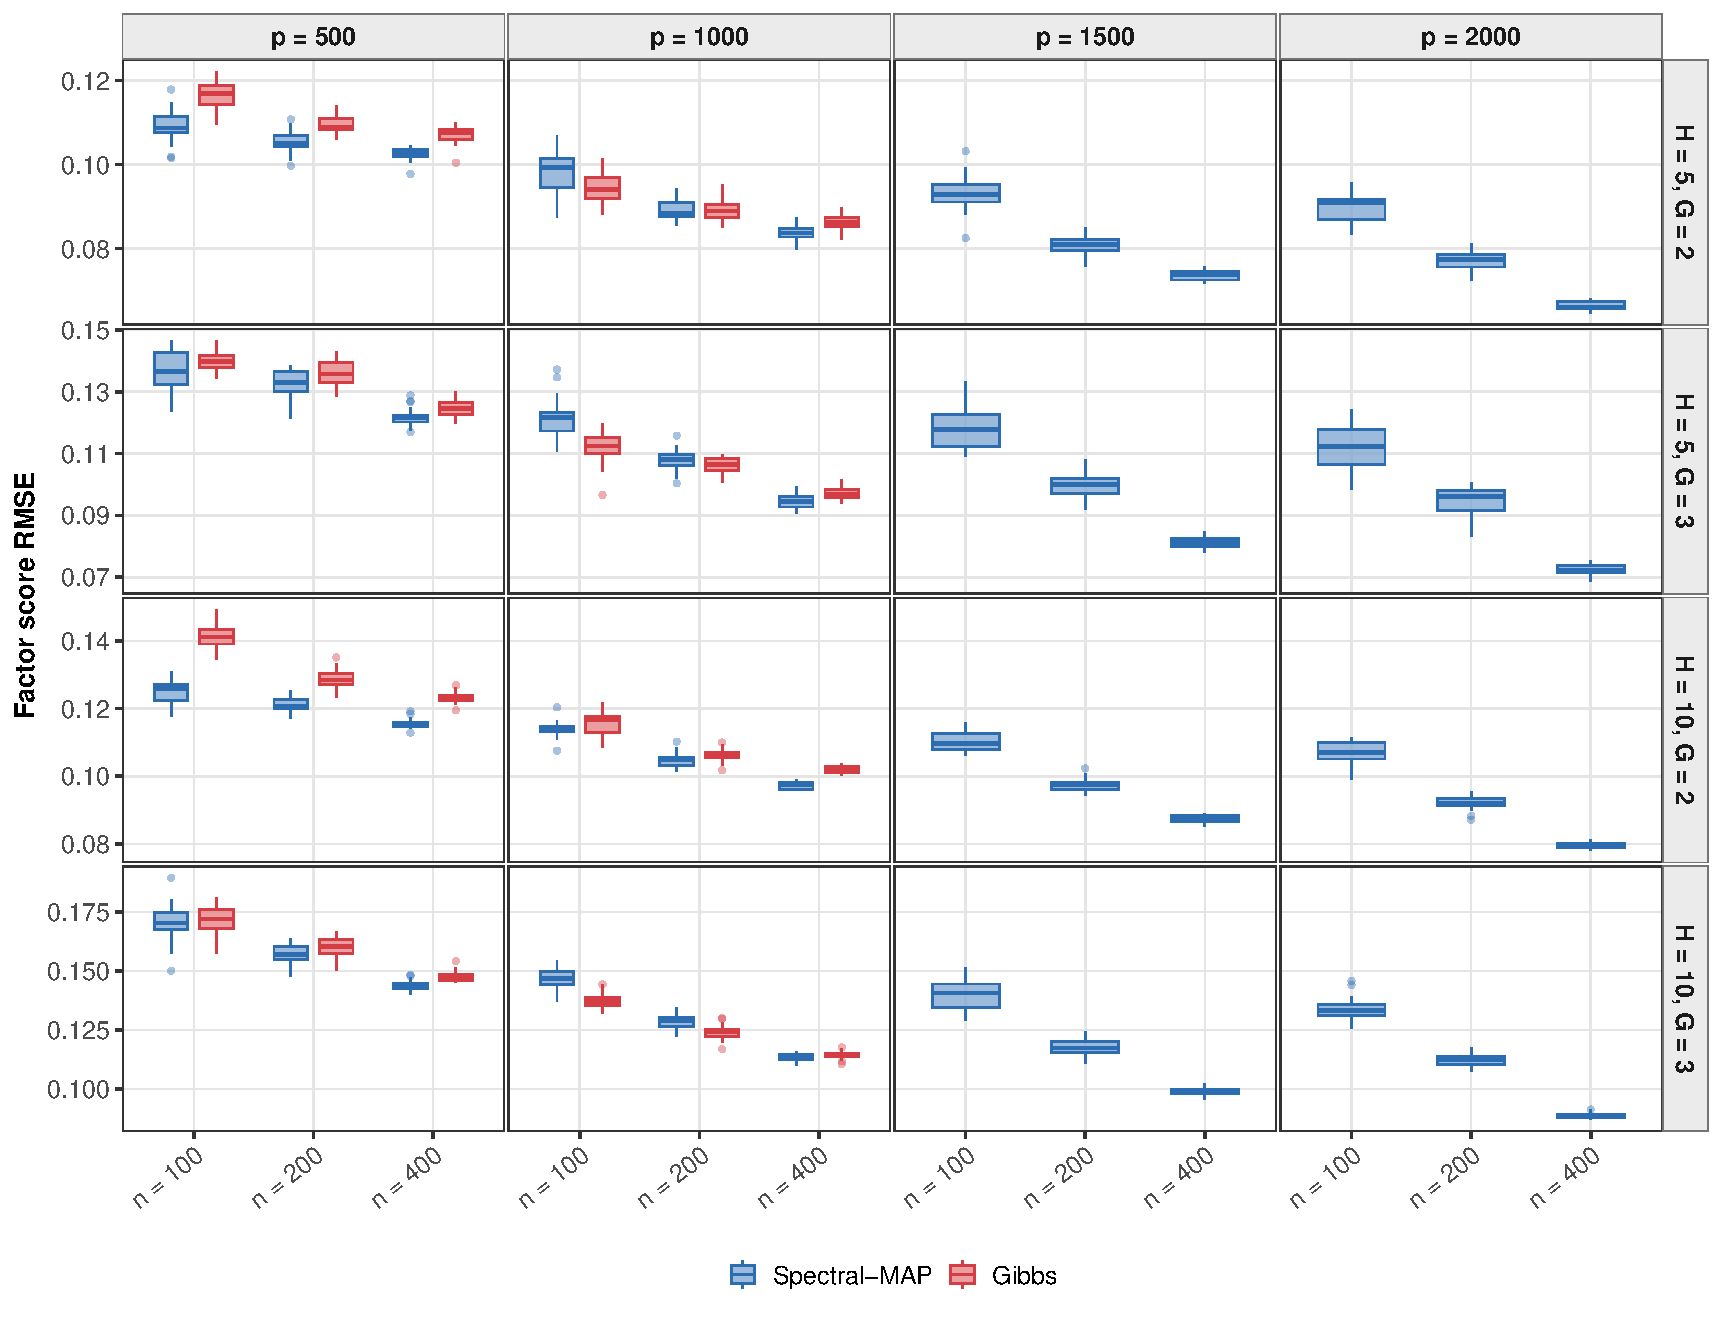
\includegraphics[width=\textwidth]{results/selected_plots/sample_size/paper_simulation_section/fig_factor_recovery_separated.pdf}
  \caption{Factor-score recovery under the separated symmetric mixture configuration. Boxplots summarize 25 replications. Gibbs was run for $p\in\{500,1000\}$; the larger-$p$ columns report Spectral-MAP.}
  \label{fig:factor_recovery_separated}
\end{figure*}

\begin{figure*}[t]
  \centering
  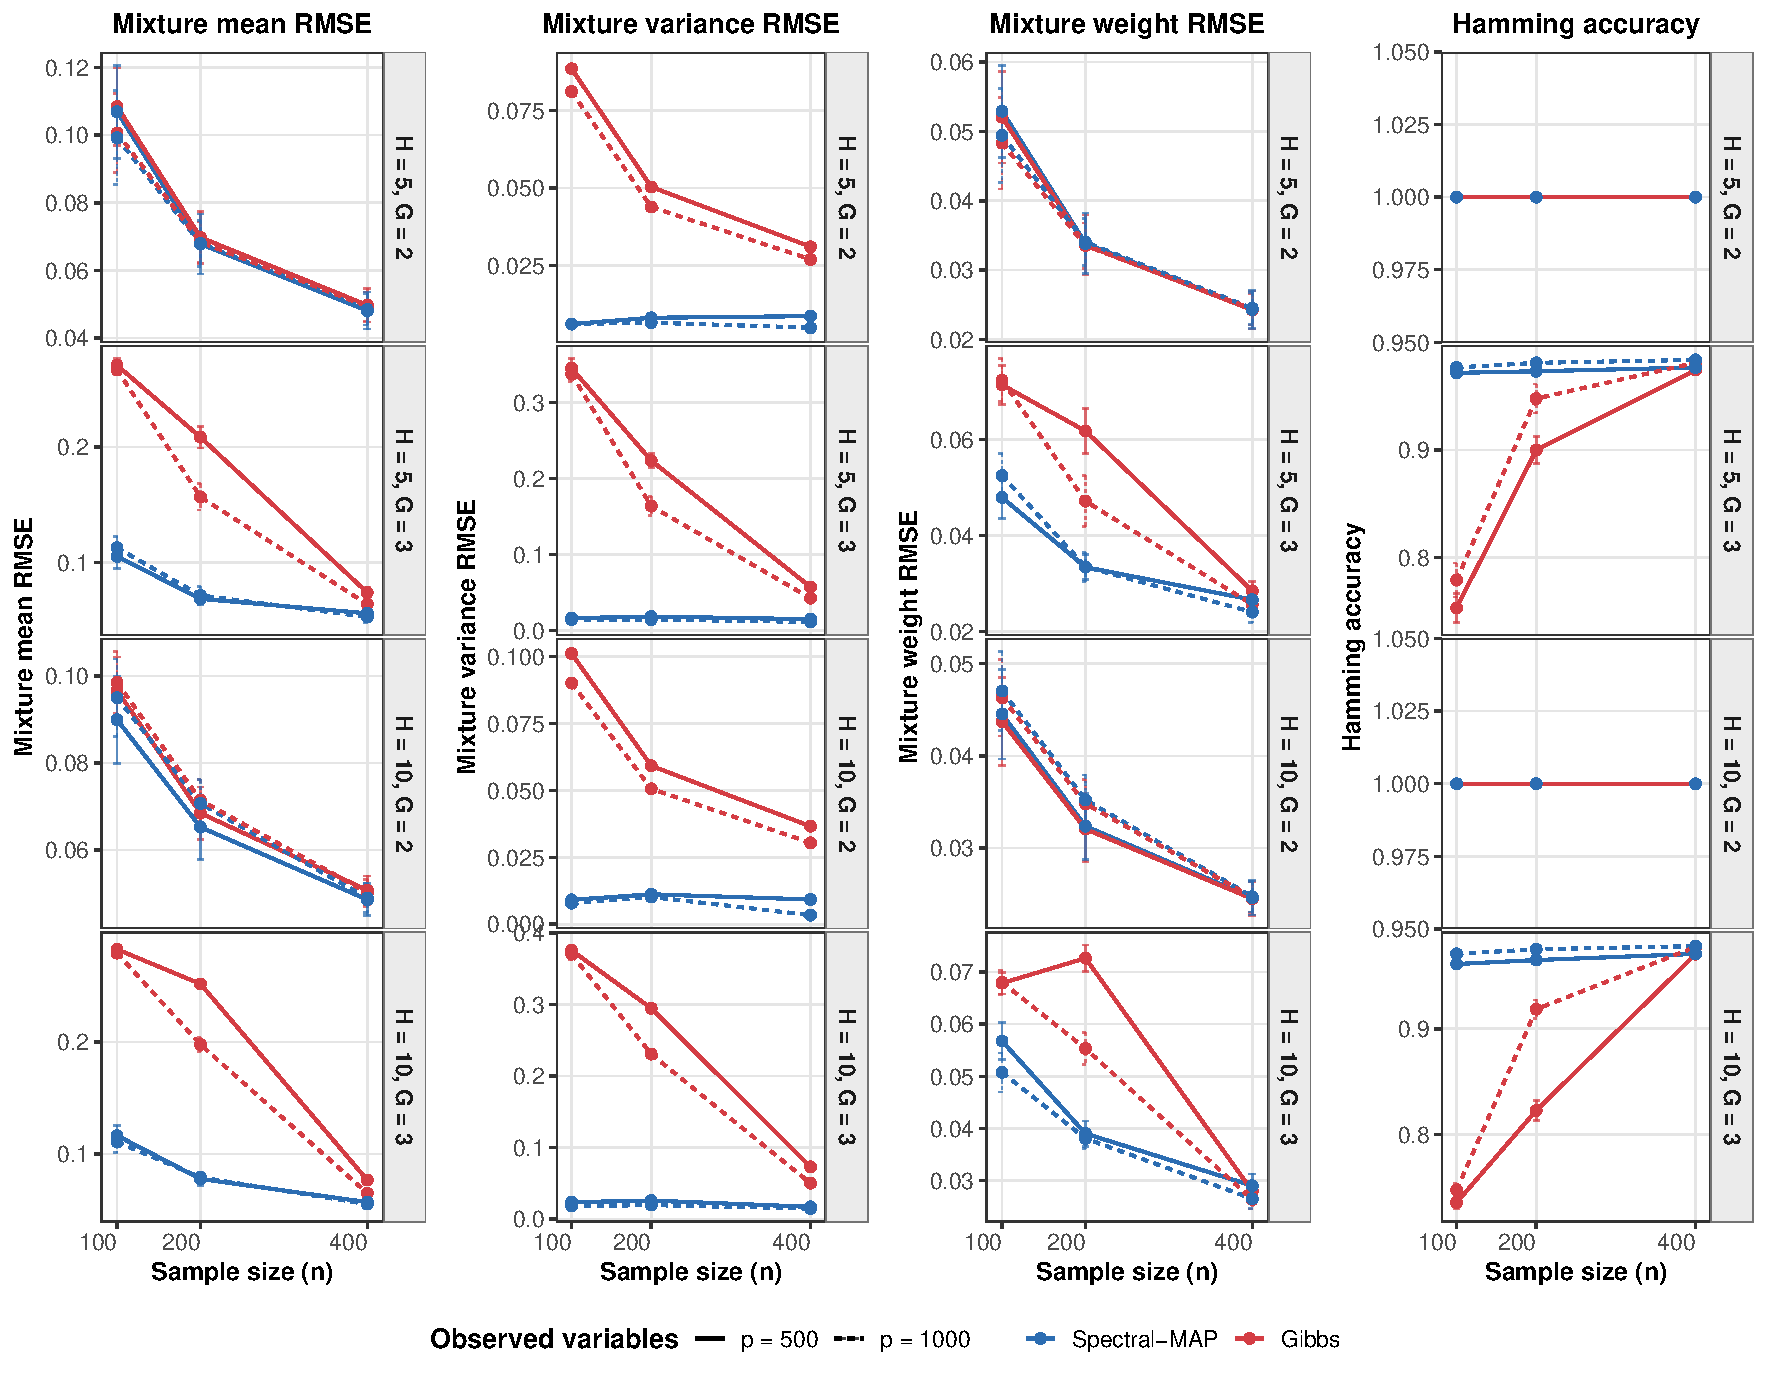
\includegraphics[width=\textwidth]{results/selected_plots/sample_size/paper_simulation_section/fig_mixture_subtype_recovery_separated.pdf}
  \caption{Mixture-parameter and subtype recovery under the separated symmetric configuration. Points are means and bars show $\pm2$ Monte Carlo standard errors over 25 replications. Line type distinguishes $p=500$ and $p=1000$. For Gibbs, Hamming accuracy uses the posterior mode of the aligned sampled allocations.}
  \label{fig:mixture_subtype_separated}
\end{figure*}

\begin{table}[t]
\centering
\caption{Subtype recovery for Spectral-MAP and two Gibbs posterior summaries. Entries are means with Monte Carlo standard deviations in parentheses, pooled over the matched $p\in\{500,1000\}$ design cells, with 25 replications per cell. The Gibbs allocation-mode estimator uses the modal aligned sampled component label for each subject and factor; the Gibbs posterior-mean plug-in estimator classifies the aligned posterior-mean score using the aligned posterior-mean mixture parameters. Higher values are better.}
\label{tab:subtype_estimators}
\begin{tabular}{llcc}
\toprule
Configuration & Subtype estimator & Hamming & Exact profile \\
\midrule
Separated symmetric & Spectral-MAP plug-in & 0.987 (0.014) & 0.908 (0.111) \\
 & Gibbs allocation mode & 0.938 (0.094) & 0.744 (0.343) \\
 & Gibbs posterior-mean plug-in & 0.971 (0.037) & 0.828 (0.218) \\
\addlinespace
Asymmetric weights & Spectral-MAP plug-in & 0.986 (0.015) & 0.902 (0.118) \\
 & Gibbs allocation mode & 0.943 (0.089) & 0.760 (0.321) \\
 & Gibbs posterior-mean plug-in & 0.968 (0.042) & 0.813 (0.233) \\
\addlinespace
Moderate overlap & Spectral-MAP plug-in & 0.953 (0.048) & 0.742 (0.273) \\
 & Gibbs allocation mode & 0.877 (0.133) & 0.588 (0.425) \\
 & Gibbs posterior-mean plug-in & 0.923 (0.080) & 0.657 (0.357) \\
\bottomrule
\end{tabular}
\end{table}


\begin{table}[t]
\centering
\caption{End-to-end computation time under the separated symmetric mixture configuration. Times are means in seconds, pooled over $n\in\{100,200,400\}$ and $p\in\{500,1000\}$, with 25 replications per design cell. Speed-up is the ratio of Gibbs time to Spectral-MAP time. ESS is the mean across replications of the median effective sample size over P-IFA parameters among the 1,000 retained Gibbs draws.}
\label{tab:runtime_comparison}
\begin{tabular}{ccrrrr}
\toprule
$H$ & $G_h$ & Spectral-MAP & Gibbs & Speed-up & Gibbs ESS \\
\midrule
5 & 2 & 20.1 & 161.2 & \textbf{8.0$\times$} & 163 \\
5 & 3 & 15.9 & 161.6 & \textbf{10.2$\times$} & 180 \\
10 & 2 & 26.8 & 218.0 & \textbf{8.1$\times$} & 159 \\
10 & 3 & 18.9 & 218.2 & \textbf{11.6$\times$} & 163 \\
\bottomrule
\end{tabular}
\end{table}

\begin{table}[t]
\centering
\caption{Oracle rotation ablation under the well-separated mixture configuration. Entries are post-refinement mean factor-score RMSE with the Monte Carlo standard deviation in parentheses, pooled over all combinations of $n\in\{100,200,400\}$, $p\in\{500,1000,1500,2000\}$, $H\in\{5,10\}$, and $G_h\in\{2,3\}$, with 25 replications per design cell ($1{,}200$ datasets). Lower values are better.}
\label{tab:rotation_ablation_separated}
\begin{tabular}{lc}
\toprule
Rotation strategy & Post-refinement factor RMSE \\
\midrule
FastICA             & $0.124\;(0.074)$ \\
FastICA + Mixture   & $\mathbf{0.109}\;(\mathbf{0.026})$ \\
Identity + Mixture  & $0.118\;(0.058)$ \\
\bottomrule
\end{tabular}
\end{table}

